% Based on format by Jos� Koiller which was updated by Daniel Foreman-Mackey

%% Use the first of the following lines during production to
%% easily spot "overfull boxes" in the output. Use the second
%% line for the final version.
% \documentclass[12pt,draft,letterpaper]{report}
\documentclass[12pt,letterpaper]{report}

\newcommand{\thesistitle}{Galaxies and Their Host Dark Matter Halos}
\newcommand{\thesisauthor}{ChangHoon Hahn}
\newcommand{\thesisadvisor}{Professor Michael R. Blanton and Roman Scoccimarro}
\newcommand{\graddate}{May 2015}

%% The following makes chapters and sections, but not subsections,
%% appear in the TOC (table of contents). Increase to 2 or 3 to
%% make subsections or subsubsections appear, respectively. It seems
%% to be usual to use the "1" setting, however.
\setcounter{tocdepth}{1}

%% Sectional units up to subsubsections are numbered. To number
%% subsections, but not subsubsections, decrease this counter to 2.
\setcounter{secnumdepth}{3}

%% Page layout (customized to letter paper and NYU requirements):
\setlength{\oddsidemargin}{0in}
\setlength{\textwidth}{6.5in}
\setlength{\topmargin}{0in}
\setlength{\headheight}{0in}
\setlength{\headsep}{0in}
\setlength{\textheight}{8.3in}
% \setlength{\footskip}{.5in}
\setlength{\skip\footins}{.3in}

\usepackage{setspace}
% \singlespacing{}
\doublespacing{}

%% This inputs your auxiliary file with \usepackage's and \newcommand's:
%% It is assumed that that file is called "definitions.tex".
\usepackage[final]{graphicx}

\usepackage{color, hyperref}
\definecolor{linkcolor}{rgb}{0,0,0.2}
\hypersetup{colorlinks=true,linkcolor=linkcolor,citecolor=linkcolor,
            filecolor=linkcolor,urlcolor=linkcolor}
\hypersetup{pageanchor=false}

\usepackage[titletoc]{appendix}
\usepackage{tocloft}
\usepackage{xpatch}

\usepackage{indentfirst}
\usepackage[tbtags]{amsmath}
\usepackage{amsfonts}
\usepackage{amssymb}
\usepackage{booktabs}
\usepackage{tabularx}
\usepackage{ctable, dashrule}
\usepackage{url}

% Custom AAS macros:
\usepackage{aas_macros}

% Bibliography:
\usepackage{natbib}
\bibliographystyle{apj}

% Algorithms:
\usepackage{algorithmic,algorithm}

% Commands:
% General formatting:
\newcommand{\paper}{Chapter}

% Foreign text:
\newcommand{\foreign}[1]{\emph{#1}}
\newcommand{\etal}{\foreign{et\,al.}}
\newcommand{\etc}{\foreign{etc.}}

% Project references:
\newcommand{\project}[1]{{\textsl{#1}}}
\newcommand{\kepler}{\project{Kepler}}
\newcommand{\terra}{\project{TERRA}}
\newcommand{\KT}{\project{K2}}
\newcommand{\tess}{\project{TESS}}
\newcommand{\jwst}{\project{JWST}}

% LaTeX object referencing:
\newcommand{\chapid}{no chapter}
\newcommand{\figref}[1]{\ref{\chapid:fig:#1}}
\newcommand{\Fig}[1]{Figure~\figref{#1}}
\newcommand{\fig}[1]{\Fig{#1}}
\newcommand{\figlabel}[1]{\label{\chapid:fig:#1}}

\newcommand{\Tab}[1]{Table~\ref{\chapid:tab:#1}}
\newcommand{\tab}[1]{\Tab{#1}}
\newcommand{\tablabel}[1]{\label{\chapid:tab:#1}}

\renewcommand{\eqref}[1]{\ref{\chapid:eq:#1}}
\newcommand{\Eq}[1]{Equation~(\eqref{#1})}
\newcommand{\eq}[1]{\Eq{#1}}
\newcommand{\eqalt}[1]{Equation~\eqref{#1}}
\newcommand{\eqlabel}[1]{\label{\chapid:eq:#1}}

\newcommand{\sectionname}{Section}
\newcommand{\sectref}[1]{\ref{\chapid:sect:#1}}
\newcommand{\Sect}[1]{\sectionname~\sectref{#1}}
\newcommand{\sect}[1]{\Sect{#1}}
\newcommand{\sectalt}[1]{\sectref{#1}}
\newcommand{\App}[1]{Appendix~\sectref{#1}}
\newcommand{\app}[1]{\App{#1}}
\newcommand{\sectlabel}[1]{\label{\chapid:sect:#1}}

\newcommand{\Algo}[1]{Algorithm~\ref{\chapid:algo:#1}}
\newcommand{\algo}[1]{\Algo{#1}}
\newcommand{\algolabel}[1]{\label{\chapid:algo:#1}}

\newcommand{\chapname}{Chapter}
\newcommand{\Chap}[1]{\chapname~\ref{chap:#1}}
\newcommand{\chap}[1]{\Chap{#1}}
\newcommand{\chapalt}[1]{\ref{chap:#1}}
\newcommand{\chaplabel}[1]{\label{chap:#1}}

\newcommand{\todo}[3]{{\color{#2}\emph{#1}: #3}}
\newcommand{\dfmtodo}[1]{\todo{DFM}{red}{#1}}

% Math:
\newcommand{\dd}{\ensuremath{\,\mathrm{d}}}
\newcommand{\bvec}[1]{{\ensuremath{\boldsymbol{#1}}}}
\newcommand{\paramvector}[1]{\bvec{#1}}
\newcommand{\unit}[1]{\mathrm{#1}}

% Probabilities:
\newcommand{\like}{\mathscr{L}}
\newcommand{\pr}[1]{\ensuremath{p(#1)}}
\newcommand{\af}{\ensuremath{a_f}}
\newcommand{\expect}[1]{\left<#1\right>}
\newcommand{\normal}[2]{\mathcal{N} (#1, #2)}

%\listfiles
%\makeatletter
%\newcommand\listofappendixname{List of Appendices}%\appendixname}
%
%\newcommand\listofappendices{%
%    \if@twocolumn
%        \@restonecoltrue\onecolumn
%    \else
%        \@restonecolfalse
%    \fi
%    \chapter*{\listofappendixname
%        \@mkboth{%
%            \MakeUppercase\listofappendixname}{\MakeUppercase\listofappendixname}}%
%    \@starttoc{toa}%
%    \if@restonecol\twocolumn\fi
%    }
%\g@addto@macro\appendix{%
%    \addcontentsline{toc}{chapter}{\appendixname}%
%    \xpatchcmd{\@part}{\addcontentsline{toc}}{\addcontentsline{toa}}{}{}%
%    \xpatchcmd{\@part}{\addcontentsline{toc}}{\addcontentsline{toa}}{}{}%
%    \xpatchcmd{\@chapter}{\addcontentsline{toc}}{\addcontentsline{toa}}{}{}%
%    \xpatchcmd{\@chapter}{\addcontentsline{toc}}{\addcontentsline{toa}}{}{}%
%    \xpatchcmd{\@sect}{\addcontentsline{toc}}{\addcontentsline{toa}}{}{}%
%    \xpatchcmd{\@sect}{\addcontentsline{toc}}{\addcontentsline{toa}}{}{}%
%}
%\makeatother
\makeatletter
    \newcommand\tableofappendices
        {\chapter*{List of Appendices}\@starttoc{toa}}
    \newcommand\l@appendix[2]
        {\par\noindent\bfseries{#1}\hfill\bfseries{#2}\par}
\makeatother


\sloppy\sloppypar


\begin{document}

%% Produces a test "layout" page, for "debugging" purposes only.
%% Comment out for final version.
% \layout  % requires package layout (see above, on this same file)

%%%%%% Title page %%%%%%%%%%%
%% Sets page numbering to "roman style" i, ii, iii, iv, etc:
\pagenumbering{roman}
%
%% No numbering in the title page:
\thispagestyle{empty}
%
\begin{center}


    \vspace*{0.5in}
    {\large\textbf{\thesistitle}}
    \vspace{.4in}

    by
    \vspace{.4in}

    \thesisauthor{}
    \vspace{.8in}
    % \vfill

    \begin{doublespace}
        A dissertation submitted in partial fulfillment \\
        of the requirements for the degree of \\
        Doctor of Philosophy \\
        Department of Physics \\
        New York University \\
        \graddate{}
    \end{doublespace}
\end{center}
\vfill

\noindent\makebox[\textwidth]{\hfill\makebox[2.5in]{\hrulefill}}\\
\makebox[\textwidth]{\hfill\makebox[2.5in]{\hfill\thesisadvisor\hfill}}
\newpage

% %%%%%%%%%%%%%% Copyright %%%%%%%%%%%%%%%%%
\vspace*{\fill}
\begin{center}
    Copyright \textcopyright\ 2017 ChangHoon Hahn \\
    This work is licensed under a Creative Commons Attribution 4.0
    International License.
    \addcontentsline{toc}{section}{Copyright}
\end{center}
\vfill
\newpage

%%%%%%%%%%%%% Blank page %%%%%%%%%%%%%%%%%%
\thispagestyle{empty}
\vspace*{0in}
\newpage

%%%%%%%%%%%%%% Acknowledgements %%%%%%%%%%%%
%% Comment out the following lines if you do not want to acknowledge
%% anyone's help...
\section*{Acknowledgements}\addcontentsline{toc}{section}{Acknowledgements}
I acknowledge people.
%Insert acknowledgement here.
%First, a huge thanks is in order for my advisor, David Hogg, for these years
%of support, encouragement, and friendship.
%I couldn't have imagined a better advisor for me and I'm looking forward to
%many years of collaboration.
%Hogg's enthusiasm is infectious and our lively discussions over lunch, coffee,
%or beer have convinced me to attempt a career in academia and made me a better
%scientist and person.
%
%I would also like to thank my other dissertation readers, Jonathan Goodman and
%Micheal Blanton, for taking the time to read my thesis and provide useful
%suggestions and clarifications that improved the presentation of this work.
%
%One of my favorite parts of studying astronomy is the community and the
%opportunities to meet and get to know amazing people from around the world.
%Over the course of my Ph.D.\ research, I have had the opportunity to
%collaborate with more people than I can possibly list here.
%I am especially grateful for the summers that I spent in Germany with Bernhard
%Sch\"olkopf and Hans-Walter Rix; the garden chats in T\"ubingen and Heidelberg
%were some of the highlights of my scientific career thus far.
%I have also enjoyed and benefited from conversations and collaborations with
%Brendon Brewer,
%Tom Barclay,
%Charlie Conroy,
%Bekki Dawson,
%Eric Ford,
%Morgan Fouesneau,
%Jonathan Goodman,
%Dustin Lang,
%Phil Marshall,
%Ben Montet,
%Tim Morton,
%Mike O'Neil,
%Adrian Price-Whelan,
%Elisa Quintana,
%Jonathan Sick,
%Dan Weisz,
%and many others.
%
%My time spent living in NYC wouldn't have been the same without my eclectic
%(and perfectly eccentric) group of housemates and friends.
%In particular, I'd like to thank Mira, Stefan, Nate, Claire, Katherine, Jacob,
%Silas, and Stumm for all the good times on Dean Street.
%I would also like to thank Ruth for being there for me when I needed her and
%sharing in life and in science, even from the opposite side of the ocean.
%
%Finally, I would like to thank my family, Annie, Clarke, and Elaine for their
%continued love, encouragement, and support every step of the way.
%I would never have made it here without them!
%
%\paragraph{Organizations}
%The results in this dissertation are based, in large part, on observations
%make by the \kepler\ Mission and subsequent \KT\ Mission with the same
%instrument.
%None of my work would have been possible without the tireless efforts of the
%scientists and engineers on the \kepler\ team.
%This work also relied heavily on the public data and literature resources
%provided by the Mikulski Archive for Space Telescopes, the NASA Exoplanet
%Archive, and the NASA Astrophysics Data System.
%
%I would like to thank the organizers and attendees of the SAMSI workshop
%``Modern Statistical and Computational Methods for Analysis of \kepler\
%Data''.
%This workshop introduced me to the \kepler\ data and drastically lowered the
%barrier to entry into the field of exoplanets.
%The connections made at this workshop have led to many important and
%long-lasting friendships and collaborations.

\newpage

%%%% Abstract %%%%%%%%%%%%%%%%%%
\section*{Abstract}\addcontentsline{toc}{section}{Abstract}
%Through the connection between galaxies and their host dark matter structures, 
Through their connection with dark matter structures, galaxies act as 
tracers of the underlying matter distribution in the Universe. Their 
%observed spatial distribution allows us to make precise measurements of large scale 
observed spatial distribution allows us to precisely measure large scale 
structure and effectively test cosmological models that explain the content, 
geometry, and history of the Universe. Current observations from galaxy 
surveys such as the Baryon Oscillation Spectroscopic Survey
have already probed vast cosmic volumes with millions of galaxies 
and ushered in an era of precision cosmology. The next surveys will 
probe over an order of magnitude more. With this unprecedented statistical 
power, the bottleneck of scientific discovery is in the methodology.
% need something that sounds better than this sentence.
In this dissertation, I address major methodological challenges in 
galaxy clustering analyses used to constrain cosmological parameters 
and investigate the connection between galaxies and their host dark 
matter structures.

%that prevent us from realizing the full potential of observations for constraining cosmology. 
Observational and instrumentational constraints present galaxy 
clustering analyses with incomplete data. Beyond restricting the 
constraining power, if not properly accounted for, these systematic 
effects significantly bias galaxy clustering measurements. I develop 
data-driven and analytic methods for robustly accounting for these
systematic effects in galaxy clustering analyses. 



I will present how major methodological challenges can be solved with robust 
treatment of systematics, higher order statistics, innovative approaches to 
probabilistic inference, and improved understanding of the galax-halo connection. 
By overcoming these challenges and unlocking the full potential the next galaxy 
surveys, I will present how we can measure the growth of structure and total 
neutrino mass with unprecedented precision.


%The study of exoplanets has been revolutionized in recent years thanks, in
%large part, to new data collected by NASA's \emph{Kepler} Mission.
%The Mission has enabled the discovery of thousands of planets orbiting stars
%throughout the Galaxy.
%These discoveries span orders of magnitude in physical parameter space but
%many of the most physically interesting questions remain open.
%The deepest of these questions is: how common are planetary systems like our
%own Solar System?
%In this dissertation, I approach this question from several different angles
%and make inferences about the frequency and distribution of planets based on
%the large, publicly-available datasets from the \emph{Kepler} and \emph{K2}
%Missions.
%
%I develop two powerful and practical methods for mining for planetary transit
%signals in the hundreds of thousands of stellar light curves measured by
%\emph{Kepler}.
%The first method is designed to find planets using the data from the
%\emph{K2} phase of the Mission where systematics introduced by the instrument
%dominate the measurements.
%Applying this method to the first publicly available dataset from \emph{K2}, I
%published more than thirty new exoplanet candidates.
%The second transit search technique is designed to find transits of planets
%with orbital periods longer than the four year baseline of the \emph{Kepler}
%Mission.
%These are interesting planets because they are expected to have the largest
%dynamical influence on the formation and evolution of their planetary systems
%but, to date, no systematic search for these signals has been published.
%I demonstrate that this method is robust and tractable and make predictions
%for the planet yields in the \emph{Kepler} dataset.
%
%I derive a general framework for making justified probabilistic inferences
%about the population of planets based on noisy and incomplete catalogs of
%exoplanet measurements.
%Applying this to a previously published catalog of exoplanets orbiting stars
%like our Sun, I measure the joint period--radius distribution of these
%planets taking into account survey selection effects and the large
%measurement uncertainties.
%Despite the fact that this catalog includes no true Earth analogs, I use the
%detected systems and weak smoothness assumptions about the underlying
%distribution to make a probabilistic estimate of the frequency of Earth-like
%planets.
%
%The main contributions of this dissertation are the development of methods for
%probabilistic and the release of open source implementations.
%One of these methods is \emph{emcee}, a method for Markov Chain Monte Carlo
%(MCMC) sampling of probability distributions.
%MCMC has been a popular method for approximate inference in astronomy for well
%over a decade but most implementations require extensive hand tuning in order
%to achieve acceptable performance on all but the simplest problems.
%Thanks to its affine-invariant sampling algorithm the \emph{emcee} method
%performs efficiently for many real problems in astronomy.
%The code has an active user base and online community of contributors.

\newpage

%%%% Table of Contents %%%%%%%%%%%%
\tableofcontents

%%%%% List of Figures %%%%%%%%%%%%%
%% Comment out the following two lines if your thesis does not
%% contain any figures. The list of figures contains only
%% those figures included withing the "figure" environment.
\newpage\addcontentsline{toc}{section}{List of Figures}
\listoffigures

%%%%% List of Tables %%%%%%%%%%%%%
%% Comment out the following two lines if your thesis does not
%% contain any tables. The list of tables contains only
%% those tables included withing the "table" environment.
\newpage\addcontentsline{toc}{section}{List of Tables}
\listoftables
\newpage

%%%%% Body of thesis starts %%%%%%%%%%%%
\pagenumbering{arabic}

%% Introduction. If your thesis has no introduction, or chapter 1 is
%% meant to be the introduction, then comment out the lines below.
\chapter*{Introduction}\addcontentsline{toc}{chapter}{Introduction}
Amidst the countless stars and galaxies we observe in the Universe lie 
undetected structures of dark matter, orders of magnitude larger than 
the luminous objects they engulf. These vast invisible structures began 
in the very early Universe, as quantum fluctuations in the aftermath of 
the Big Bang. 
%These vast invisible structures began as quantum fluctuations in the beginning of the Universe in the aftermath of the Big Bang. 
During the subsequent period of inflation (\todo{cite?}), these primordial fluctations 
were amplified by the accelerated expansion of the Universe and then 
propagated through gravitational instability for billions of years. 

Despite constituting most of the matter in the Universe, dark matter 
has yet to be directly observed. In fact, it can only be studied through 
its gravitational interactions with luminous baryons — the matter that 
constitutes stars, galaxies, and celestial objects that emit light. 
In a way, the galaxies we observe in the cosmic volumes probed by our 
telescopes act as illuminated beacons tracing the vast dark matter 
terrains of the Universe.

Over the past decade, spectroscopic redshift surveys like the 
Baryon Oscillation Spectroscopic Survey (BOSS\todo{cite}) have 
exploited these galactic beacons to map out the cosmic structure
of the Universe. Precise measurements of distance and growth 
of large-scale structure (LSS) from these surveys, provide tests 
of cosmological models that describe the content, geometry and history 
of the Universe. \todo{By analyzing measurements of LSS,}


Through these galaxies, we can explore the properties of the underlying dark matter
and the growth of their structure. Measurements that quantify these properties allow us to make
precise calculations of cosmological parameters, which quantify the content, geometry, and
expansion history of the Universe. Ultimately the constraints we measure on these parameters,
enlighten us on the properties of dark energy, which remains one of the most crucial unsolved
questions in cosmology. Certainly these precise cosmological measurements require a profound
understanding of the formation and evolution of galaxies. Unfortunately there is no clear
narrative of galaxy formation and evolution due to the complex, non-linear, and stochastic nature
of the physical processes that govern them.

In fact, galaxy formation and evolution remain another central unsolved questions in
astrophysics and cosmology. However, since galaxies are enveloped in the massive gravitational
wells of their host dark matter structures, the underlying dark matter of galaxies undoubtedly
plays a crucial role in their formation and evolution. Therefore, with its implications on the most
crucial questions in both cosmology and our understanding of galaxies, the interactions between
galaxies and their host dark matter environments pose some of the most impactful questions,
questions that I seek to answer in my dissertation. 


\section{Large Scale Structure in $\Lambda$CDM} \label{sec:lss}
From the early Universe, primordial quantum fluctuations grow into the 
large-scale structures of the Universe we observe today through gravitational 
instability over the different epochs of cosmic history. In this section, I briefly 
describe the simplified ({\em linear}) theory of this evolution and explain core 
concepts of LSS cosmology using galaxies. Lets begin by defining the matter 
overdensity field (or density fluctuation) at comoving position ${\bf r}$: 
\beq \label{eq:delta}
\delta({\bf r}) = \frac{\rho({\bf r}) - \bar{\rho}}{\bar{\rho}}, 
\eeq
where $\rho({\bf r})$ and $\bar{\rho}$ are the density field and mean 
density respectively. In Fourier space ($k$-space), Eq.~\ref{eq:delta} can 
be Fourier transformed, 
\beq
\delta({\bf k}) = \int \frac{{\rm d^3}{\bf r}}{(2\pi)^3} e^{-i{\bf k}\dot{\bf r}}\;\delta({\bf r}).
\eeq
For describing the evolution of the overdensity field, Fourier space is generally 
favored over configuration space because, as derived later in the section,
the Fourier modes of $\delta$ evolve independently in linear theory -- 
\emph{i.e.} on large scales.

The information in the overdensity field is often quantified using its 
$N$-point statistics (\todo{cite Peebles bernardeua}). In fact, the two-point
statistic is one of commonly used tool in large scale structure studies.
This two-point statistic (also referred to as the correlation function) is
defined as, 
\beq
\xi(r) = <\delta({\bf x})\delta({\bf x} +  {\bf r})>
\eeq
and in Fourier space as,
\beq
<\delta({\bf k})\delta({\bf k'})> = (2\pi)^3 P(k) \delta^{D}({\bf k}+{\bf k'}).
\eeq
$\delta^{D}$ is the Dirac delta function and $P(k)$ is the {\em powerspectrum}, 
the Fourier transform of $\xi$. In principle, $\xi$ and $P(k)$ contain the same 
information. In practice, however, analyzing $\xi$ versus $P(k)$ carry different 
caveats (\todo{cite FKP}). Throughout this section, and also the dissertation, 
I will mainly focus on the powerspectrum. 

The evolution of the dark matter overdensity field can be derived (on 
sub-horizon scales) as follows. For pressureless dark matter, the equation of motion
can be derived from the continuity, Euler, and Poisson equations
\beqa 
\frac{\partial \rho}{\partial t} + \nabla \dot \rho {\bf u} = 0  \\ 
\frac{\partial {\bf u}}{\partial t} + ({\bf u} \dot \nabla) \dot {\bf u} - \nabla\Phi = 0 \\ 
\nabla^2\Phi - 4 \pi G \rho = 0 
\eeqa
to 
\beq \label{eq:meszaros}
\frac{\partial^2 \delta}{\partial t^2} + 2 \frac{\dot{a}}{a} \frac{\partial \delta}{\partial t} - 4 \pi G \bar{\rho} \delta = 0.
\eeq
${\bf u}$ is the velocity field, $\Phi$ is the gravitational potential, and $a$ 
is the scale factor. For a detailed derivation I refer readers to \todo{cite Peebles 
or Dodelson}. Eq.~\ref{eq:meszaros} a second order differential equation, therefore,
the solution can be written as 
\beq 
\delta({\bf r}, t) = D^{(+)}(t) A({\bf r}) + D^{(-)}(t) B({\bf r}).
\eeq
The density flucation has two components: a growing mode $D^{(+)}$ and a decaying 
mode $D^{(-)}$. The decaying mode decreases with time and its contribution becomes negligible
leaving only the growing mode in the late Universe. Now in order to quantify
the evolution of the growing mode $D^{(+)}$, one commonly used quantity is the 
``growth rate of structure'': 
\beq \label{eq:f_growth}
f = \frac{ d {\rm ln}\;D^{(+)}}{d {\rm ln}\;a}. 
\eeq
This growth rate of structure is a key quantity in LSS cosmology for testing different 
cosmological models and theories of gravity. $f$ will be discussed further in Section~\ref{sec:rsd}.

From the early Universe the density fluctuations evolve through different epochs in 
cosmic history: inflation, radiation-dominated, and matter-dominated eras. Each of 
these periods leave an imprint on the evolution of $\delta$. Fig.~\ref{fig:lifo}, 
marks the different eras in the early Universe and plots how the physical scale of 
the Universe, represented by the Hubble radius, evolves with $a$. 

During inflation, the Hubble radius remains constant. Afterwards the Universe 
becomes radiation dominated. Based on the Friedmann equations the Hubble radius 
during the radiation dominated era is approximately $\propto a^{2}$. The Universe then 
becomes matter dominated and the Hubble radius is approximately $\propto a^{3/2}$. 
Meanwhile, the physical scale of perturbations is 
$\lambda_{phys} = \lambda_{comov}\ a(t) \propto a(t)$. As Fig.~\ref{fig:lifo} 
illustrates, perturbations exit the Hubble radius during inflation then 
reenter the Hubble radius later on. Depending on the physical scale of the 
perturbation, it can enter either during the radiation dominated  
(smaller scale) or matter dominated (larger scale) era. 


The physical scale of perturbations that enter the horizon at the time of 
matter-radiation equality ($a(t) = a_{eq}$), $\lambda_{eq}$ is $\sim 500 h^{-1}Mpc$.
The perturbations that enter before the matter-radiation equality during 
the radiation dominated era, have physical scales $\lambda_{phys} < \lambda_{eq}$. 
These smaller scale perturbations, todo{explain the supression} 
On the other side, the larger scale perturbations with $\lambda_{phys} > \lambda_{eq}$
enter after matter-radiation equality during the matter dominated epoch. These 
perturbations do {\em not} experience the suppression of growth of the radiation 
dominated era. Therefore, as the overdensity field goes through these epochs, its 
growth on small scale is suppressed by a factor of $\sim k^4$.  


In practice, this scale dependent evolution of the density fluctuation is 
quantified through the ``transfer function'' $T(k)$ (\todo{cite all the transfer function papers}). After inflation the 
powerspectrum of the density fluctation can be summarized by: 
\beq
P_{\rm inf}(k) \propto k^{n_s}
\eeq
where $n_s \sim 1$ \todo{cite inflation papers: Harrison (1970), Zel’dovich (1972) and Peebles Yu (1970) Komatsu et al. 2011}. Then powerspectrum of the density 
fluctuation in the late Universe can be expressed as 
\beq
P(k) \propto k^{n_s} \; T^2(k) \; D^2(k). 
\eeq
$D(k) \equiv D^(+)$ from earlier this section. 

\begin{figure*}
\begin{center}
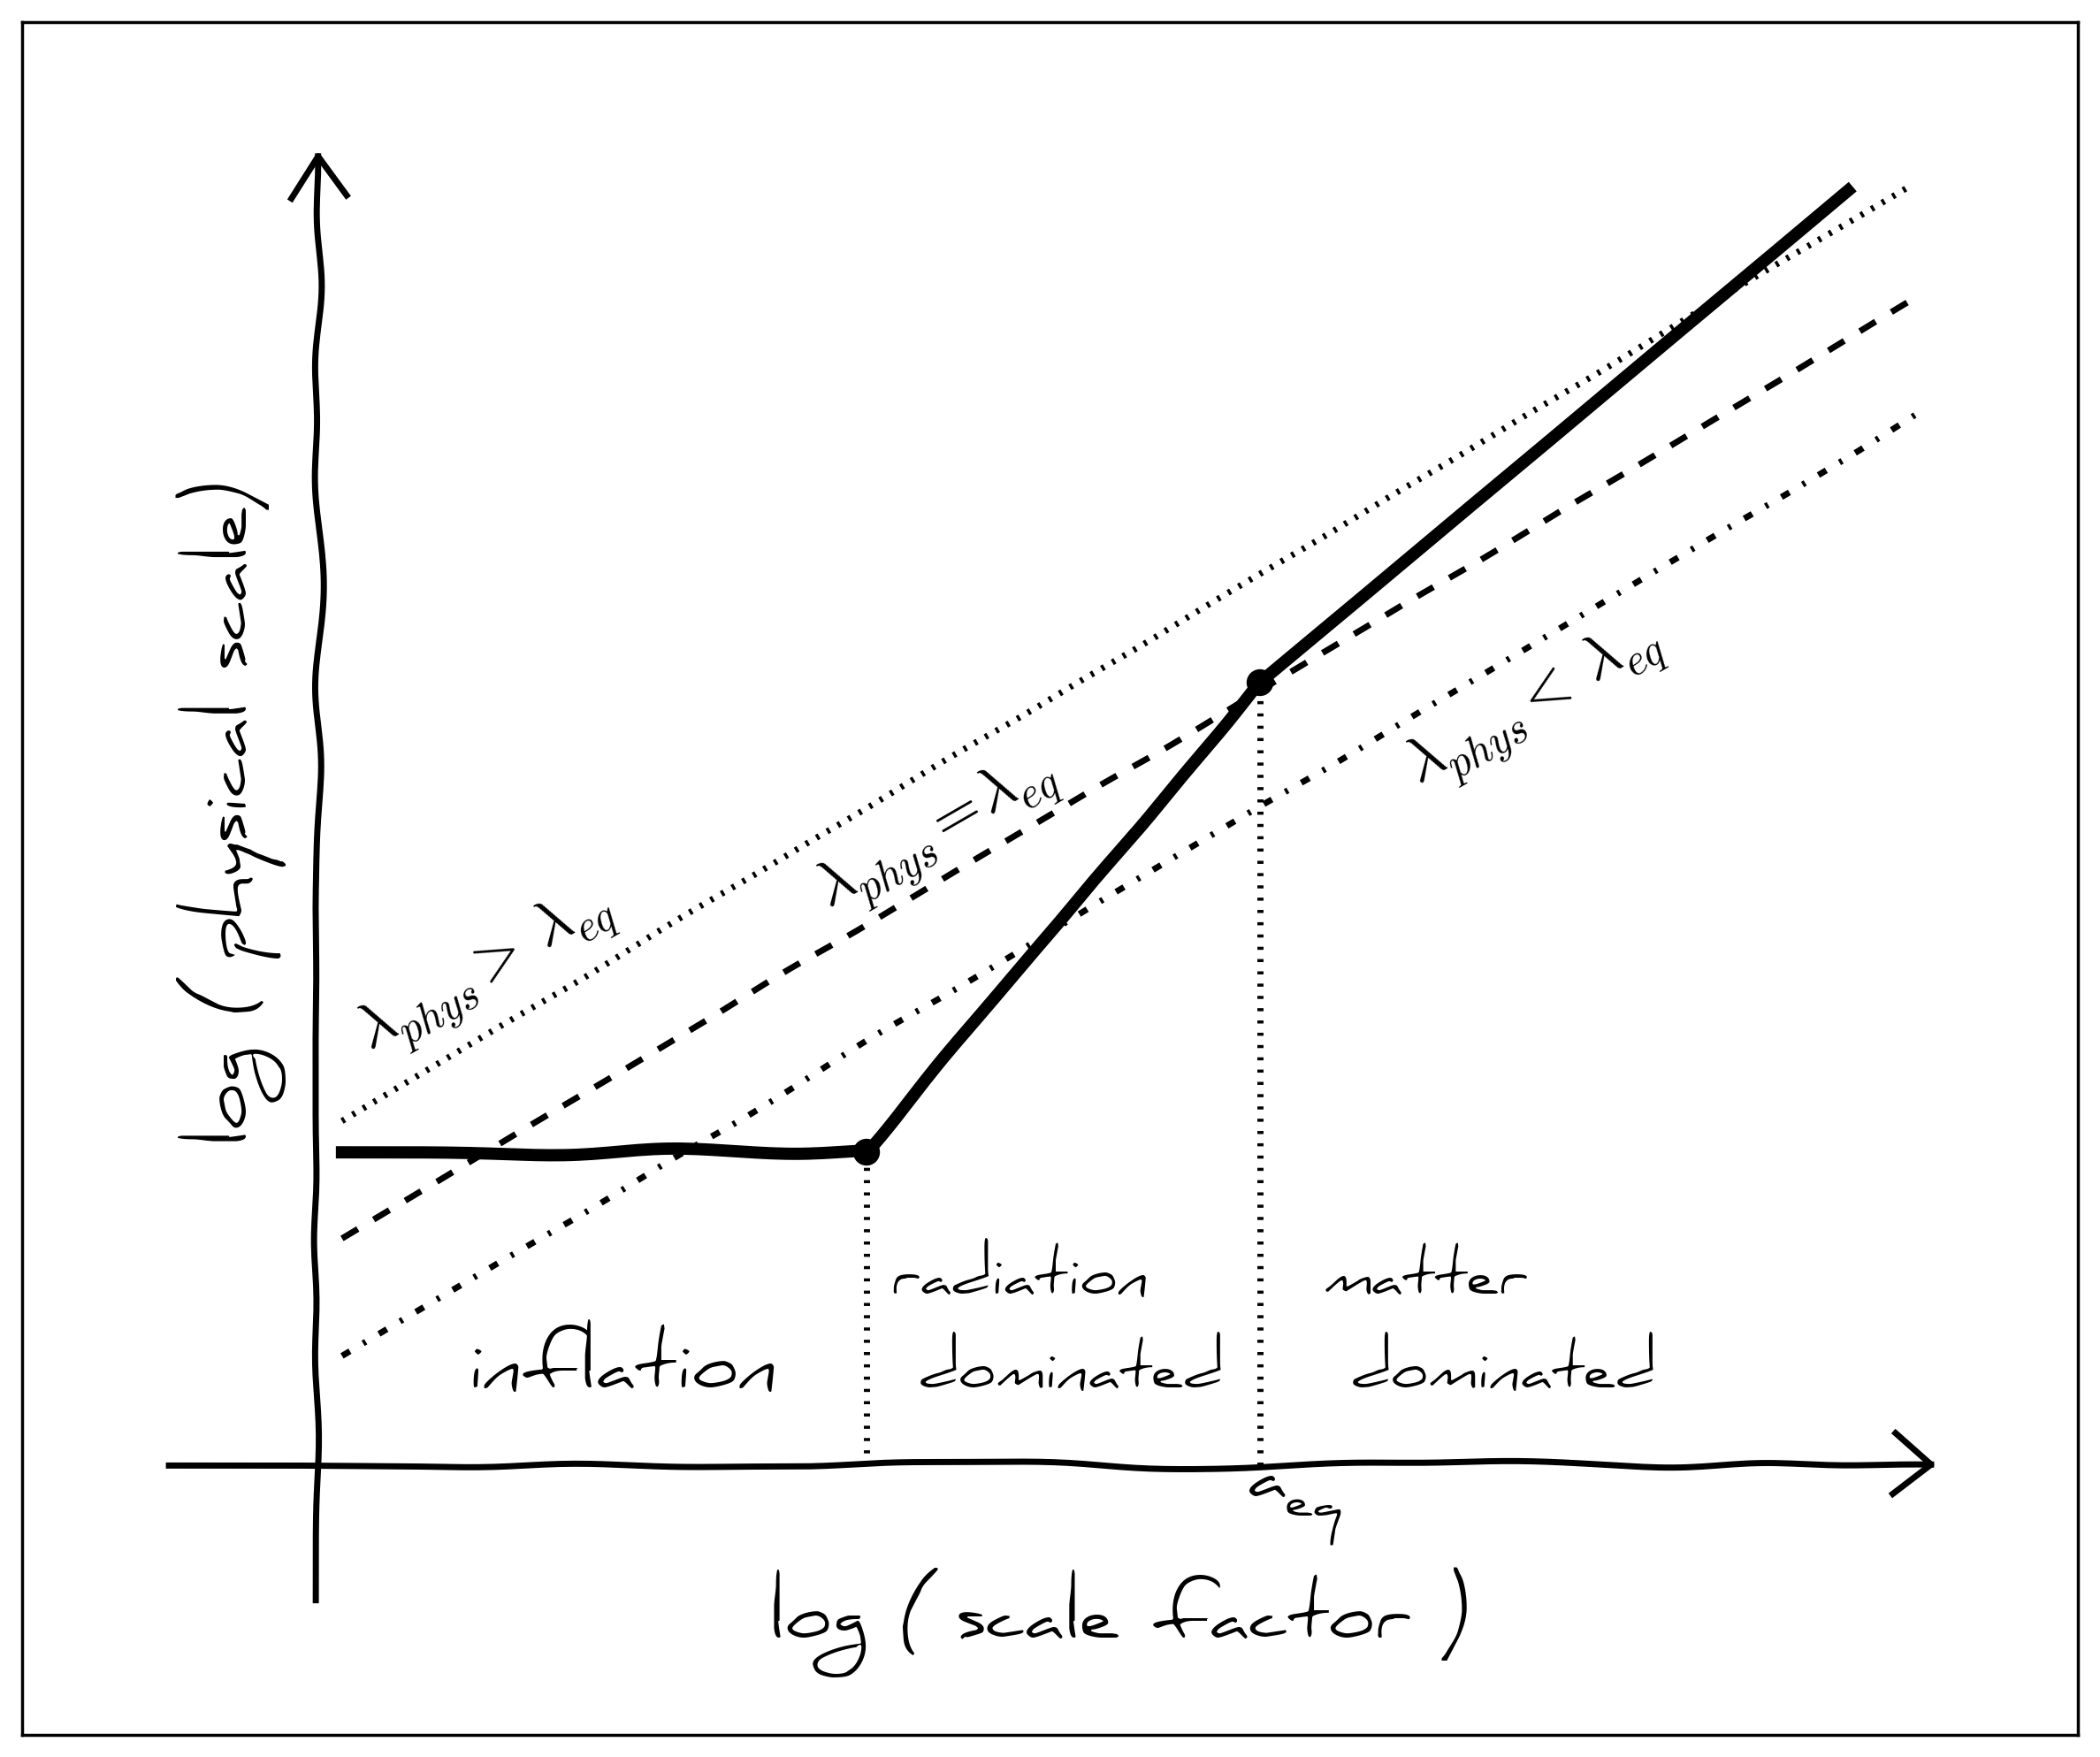
\includegraphics[width=\textwidth]{figs/lifo.png}
\caption{Schematic diagram that illustrates the evolution of the Hubble radius
(Above) The evolution of the Hubble radius (solid line) during inflation (flat), radiation
domination, and matter domination (note inflection). Dashed, dotted, and dot-dashed
lines show the physical length of three constant comoving scales. The scale corresponding
to the current Hubble radius cH−1
0 first “left the horizon” about 60 e-folds before the end
of inflation (open circle).
} \label{fig:lifo}
\end{center}
\end{figure*}

\todo{paragraph about how because D and T depend on cosmological parameters 
    so powerspectrum measurements of the matter density fluctuation can be 
    used a tests of the cosmological models.
}
So powerspectrum measurements of the matter density fluctuations can be compared
to predictions of various cosmological models in order to produce constraints 
on cosmological parameters, better understand dark energy, and test theories of 
gravity. Unfortunately, most of the matter in the Universe is in the form of dark 
matter and does not interact with radiation. 

Observers cannot measure the spatial statistics (or clustering) of dark matter 
directly. Instead, we measure the clustering of galaxies and quasars, which trace
the underlying matter distribution. The smoothed galaxy/quasar density field is 
approximated by a local function of the matter density field
\beq
\delta_g({\bf r}) = F( \delta({\bf r} ). 
\eeq
This function can then be expanded Taylor series,
\beq
\delta_g({\bf r}) = \sum\limits_{k=0}^{\infty} \frac{b_k}{k!} \delta^k. 
\eeq
$b_1$ is referred to as the linear bias factor and $b_0$ is chosen so that
$<\delta_g> = 0$. To linear order, 
\beq
P_g(k) = b_1^2 P(k). 
\eeq
The primary subpopulation of galaxies used so far for LSS studies are luminous 
red galaxies (\todo{Eistenstien apper}). These galaxies have $b_1 > 1$, which 
means they are {\em biased} tracers of the matter distribution (\todo{cite Zehavi 2005, Sheldon 2009, Gastanage 2009}). 
This bias is caused by the fact that luminous galaxies reside in larger potential 
wells, which have stronger clustering properties than than less massive ones (\todo{manera 2010}). 

Based on the simplified derivation of this section, once we have the spatial 
distribution of galaxies or quasars we can derive the clustering of the matter
distribution and then infer cosmological constraints. In practice, however, a
number of factors complicate this procedure. One key complication is redshift-space
distortions, which will be discussed in the following section.

\section{Redshift-Space Distortions} \label{sec:rsd}
Spectroscopic redshifts surveys, such as 2dFGRS, SDSS, and BOSS, have mapped out
millions of distant galaxies. Current surveys such as Extended Baryon Oscillation 
Spectroscopic Survey (eBOSS; \citealt{Dawson:2015aa}), and future surveys such as 
the Dark Energy Survey Instrument (DESI; \citealt{Schlegel:2011aa, Morales:2012aa, Makarem:2014aa}) 
and the Subaru Prime Focus Spectrograph (PFS; \citealt{Takada:2014aa}), will 
continue to map out millions more. These surveys dominate LSS studies and have/will 
been critical for inferring precise cosmological constraints. As their name suggest, 
however, these {\em redshift} surveys do not directly measure the position of 
galaxies, but rather the angular positions (right ascension and declination) and
redshift of galaxies. 

Redshifts from spectroscopic surveys observe the combination of recession 
velocities due to the expansion of the Universe and the peculiar velocities of the galaxies 
\beq
z_{obv} = z_{true} +  \frac{v_{pec}}{c}.
\eeq 
The comoving positions derived from the angular positions and redshifts are then
in {\em redshift-space} and ``distorted'' compared to real-space comoving positions:
\beq
{\bf s} = {\bf x} +  \frac{{\bf v}_{pec} \cdot \hat{n}}{H_0}.
\eeq 
$\hat{n}$ is the unit vector along the line-of-sight. Thankfully, all hope is not 
lost. The peculiar velocities of galaxies should be directly related to the total 
matter distribution, since galaxies can be thought of as test particles in a 
gravitational field. 

\todo{Kaiser 87} derives an approximation for the distortion caused by the coherent 
infall of galaxies onto over dense regions in redshift space. This redshift-space 
distortion (RSD), often referred to as the Kaiser effect, causes overdense regions
to appear squashed along the line of sight in redshift space. Galaxies around an
overdense region closest to the observer (us) are moving towards the center of the 
overdense region, so they appear in redshift-space to be farther away. Galaxies 
on the other side of the overdense region are moving towards it and the observer, 
so they appear closer to us. 

More precisely, the relation between the overdensity field in redshift-space can be 
derived from the continuity equation and the distant observer approximation, 
\beq
\delta^{(s)}({\bf k}) = (1 + f \mu^2) \delta({\bf k}).
\eeq
$f$ here is the growth rate of structure from Eq.~\ref{eq:f_growth} and 
$\mu = {\bf k} \cdot \hat{n} / k$, cosine of the angle between $k$ and 
the line of sight. 

The Kaiser effect can be combined with the galaxy bias model from 
Section~\ref{sec:lss}, in order to express the galaxy overdensity field in 
redshift-space:
\beq
\delta_g^{(s)}({\bf k}) = (b + f \mu^2) \delta({\bf k}).
\eeq
The redshift-space powerspectrum of the galaxy overdensity field can then be
written as 
\beq
P_g^{(s)}(k, \mu) = (b + f \mu^2)^2 P(k).
\eeq
On large scales and with small overdensities, the effect of redshift-space 
distoritons is well described by the Kaiser effect. On small scales with large
overdensities things get a little more complicated. 

The random peculiar velocities of galaxies in gravitationally bound structures 
such as clusters cause their position in redshift-space along the line-of-sight 
to be smeared out to larger scales.  This effect can easily be identified by 
eye in galaxy redshift maps. The elongations of the galaxy positions along the 
line-of-sight look like fingers pointing towards the observer. Hence this 
redshift-space distorion is called the ``fingers-of-god''. Its impact on the 
powerspectrum, is typically quantified using an overall exponential factor such as 
\beq
P_g^{(s)}(k, \mu) \approx e^{-f^2 \sigma_v^2 \mu^2 k^2} (b + f \mu^2)^2 P(k).
\eeq
$\sigma_v$ is a paramter quantifying the strength of the effect and is usually
left as a free parameter. 

The relations that quantify the impact of RSDs reveal another means of measuring 
$f$. Consider the Legendre expansion of $P_g^{(s)}(k, \mu)$, 
\beq
P_g^{(s)}(k, \mu) = \sum\limits_{\ell=0, 2, 4 ...} \mathcal{L}_\ell(\mu) P_g^\ell(k). 
\eeq
Each of the powerspectrum ``multipoles'' of this expansion can be written as 
\beq
P_g^{\ell}(k) = \frac{2 \ell + 1}{2} \int\limits_{-1}^{1} {\rm d}\mu \; P_g^{(s)}(k, \mu) \mathcal{L}_\ell(\mu).
\eeq
The powerspectrum multipoles for $\ell= 0$ (monopole) and $2$ (quadrupole), neglecting 
the figers-of-god which does not significantly impact larger scales, are
\beqa
P_g^0 (k) = (b_1^2 + \frac{2}{3} f b_1 + \frac{1}{5}f^2) P(k) \\
P_g^2 (k) = (\frac{4}{3} f b_1 + \frac{4}{7} f^2) P(k). 
\eeqa
Their ratio 
\beq \label{eq:multipole_ratio}
\frac{P_g^2}{P_g^0} = \frac{\frac{4}{3} f b_1 + \frac{4}{7} f^2}{b_1^2 + \frac{2}{3} f b_1 + \frac{1}{5}f^2},
\eeq
illustrates how the distortions caused by RSDs allow us to extract information of 
$f$ through measurements of the redshift-space galaxy powerspectrum!  

\section{Weighting Neutrinos with Galaxies} \label{sec:mneut}
Beyond providing a way to infer the growth rate of structure, which 
can be used to test GR and modified gravity scenarios, galaxy clustering
also provides a unique window to probe fundamental physics beyond the 
standard model. 
In the derivations of Sections~\ref{sec:lss} and~\ref{sec:rsd} we focused 
on how the density fluctuations of dark matter evolves. Because dark matter 
consistutes majority of the matter in the Universe, this is an excellent 
approximation. However, it negelects some of the more detailed imprints on 
large-scale structure from other matter components-- \emph{i.e.} neutrinos. 
Oscillation and detection experiments have (\emph{very} Nobel Prize in Physics 2015) 
convincingly confirmed {\em not} massless (\todo{Beringer et al. 2012,Lesgourges, 2012, 2013})

In the very early Universe, neutrinos are relativistic and coupled to the 
primordial plamsa. Later they decouple from the plasma, while they are still 
ultra-relativistic and redshift. While they are relativistic, they do not 
contribute to the energy density of matter but instead radiation. Then during 
matter domination, neutrinos eventually become non-relativistic. At this point, 
neutrinos contribute to the matter energy density and act as ``warm/hot'' 
dark matter.

Neutrinos after they decouple from the primoridal plasma constitutes a 
collisionless fluid, where the individual particles free-stream with 
characteristic velocities defined by their thermal velocity. While 
neutrinos are relativistic, their free-streaming scale is simply 
equal to the Hubble radius. But when they become non-relativistic, 
their can be expressed as
\beq
v_{\rm th} \approx 158 (1 + z) \left(\frac{1 {\rm eV}}{m} \right) \; \; {\rm km \; s^{-1}}
\eeq
and the free-streaming scale can be derived in an analogous way as
Jean's length
\beq
\lambda_{\rm FS} = 2 \pi \sqrt{\frac{2}{3}} \left( \frac{v_{\rm th}}{H} \right)
\eeq
or 
\beq \label{eq:kfs}
k_{\rm FS} = \frac{2\pi a}{\lambda_{\rm FS}} \approx  0.82 \frac{\sqrt{\Omega_\Lambda + \Omega_m(1+z)^3}}{(1+z)^2} \left(\frac{m_\nu}{1\;{\rm eV}} \right).
\eeq
$\Omega_\Lambda$ and $\Omega_m$ are the current cosmological constant and matter 
density fractions, respectively.

Neutrinos leave two main imprints on LSS. In the early Universe they contribute
to the radiation energy density. After they become non-relativistic in matter
domiation, they contribute to the matter energy density. As described in 
Section~\ref{sec:lss}, matter-radiation equality marks the turning point in 
suppression of growth of structure, quantified by $T(k)$. The transition of 
neutrinos from radiation to matter impacts $a_{eq}$ and thus shifts the turning 
point of the cold dark matter (CDM) only powerspectrum. 
Even after becoming non-relativistic, neutrinos do not contribute to the
clustering of matter on scale smaller than the free-streaming scale, 
$k_{\rm FS}$ (Eq.~\ref{eq:kfs}). The impact of this scale dependent 
suppression of clustering, can be analytically estimated for the powerspectrum: 
\beq
\frac{\Delta P}{P} = \frac{P^{f_\nu \neq 0} - P^{f_\nu = 0}}{P^{f_\nu = 0}} \approx - 8 f_\nu \;\;\;\; {\rm for}\;\; k \gg k_{\rm FS}.
\eeq
$f_\nu = \Omega_\nu / \Omega_m$.

The total mass of neutrinos (\mneut) dictate the strength of these imprints. 
The broadband shape of the powerspectrum offers a unique opportunity to measure
the extent of these imprints and constrain \mneut. The same tools that we 
use for analyzing RSDs and measuring the growth rate of structure can be used 
to measure \mneut from observations of galaxy surveys.
Based on their forecasts (DESI; \todo{cite}), the next galaxy surveys have the
potential to infer the most stringent constraints 
($\sigma_{\sum m_\nu} \sim 0.03\;{\rm eV}$) on \mneut. Such constraints would 
trump those from particle physics experiments (\todo{Wolf}) and have the potential to distinguish
between the normal or invereted neutrino mass hierarchy and reveal physics
beyond the Standard Model.

\section{Analyzing Galaxy Clustering}
%Beyond the general description and derivation of the redshift-space galaxy powerspectrum, the rest of galaxy clustering analysis in LSS studies follows the standard approach to Bayesian parameter inference. 
The ultimate goal of galaxy clustering analyses is to derive constraints on cosmological 
parameters and models from observed measurements of galaxly clustering -- the probability 
distribution of the cosmological parameters (\emph{e.g.} $f$, \mneut) given observations. 
The standard approach to deriving this {\em posterior} probability distribution is using 
Bayesian parameter inference. Based on Bayes theorem, the posterior probability distribution 
can be expressed as 
\beq
P({\bf \theta}| {\bf D}) = \frac{P({\bf D}|{\bf \theta}) P({\bf \theta})}{P({\bf D})}.
\eeq
${\bf D}$ and ${\bf \theta}$ refer to observations and cosmological parameters, respectively. 
$P({\bf D}|{\bf \theta})$, the probability distribution function for the observation ${\bf D}$ 
given model parameters ${\bf \theta}$ -- {\em i.e. likelihood function}, $\mathcal{L}$. 
$P({\bf \theta})$ is the {\em prior} probability distribution function. Lastly, $P({\bf D})$ 
is the ``evidence'', which for our purposes, is just a normalization factor independent of
${\bf theta}$. More commonly the equation above is more simply written 
\beqa \label{eq:bayes} 
P({\bf \theta}| {\bf D}) &\propto& P({\bf D}|{\bf \theta}) P({\bf \theta}) \\
{\rm posterior} &\propto& {\rm likelihood}\; \times \; {prior}.
\eeqa

In the context of galaxy clustering analyses and LSS cosmology in general, the likelihood 
function is {\em typically} assumed to have Gaussian function form and calculated as 
\beq \label{eq:likelihood}
P({\bf D}|{\bf \theta}) = \mathcal{L} = \frac{1}{(2\pi)^{N_d/2}\; {\rm det}{\bf C}^{1/2}}\; {\rm exp}\left[ -\frac{1}{2} ({\bf D} - F({\bf \theta}))^T {\bf C}^{-1} ({\bf D} - F({\bf \theta}))\right].
\eeq
${\bf D}$ is data from observations with dimension $N_d$. $F({\bf \theta})$ is the model prediction 
of the observable generated from cosmological parameters ${\bf \theta}$. And ${\bf C}$ is 
the covariance matrix. ${\bf D}$ is observed and measured from galaxy surveys. $F({\bf \theta})$
is broadly described by the derivations earlier this section. The covariance matrix ${\bf C}$
can be estimated using a number of different methods. 

Efforts to analytically estimate the covariance matrix from theory have been made in the past
(Hamilton, Rimes Scoccimarro 2006; Sefusatti et al. 2006; Pope Szapudi 2008; de Putter et al. 2012). 
Non-linear evolution, shot-noise, RSDs, and mapping between galaxies and matter, however,
complicate accurate estimations. Jack-knife resampling is another method for estimating 
covariances -- directly from data (Krewski 1981; Shao and Tu 1995). However, the method 
requires a number of arbitrary choices and cannot account for fluctuations on the scale 
of the survey (Norberg 2009). Instead, the latest analysis have estimated the ${\bf C}$ 
from a large number of galaxy mock catalogs generated from $N$-body simulations. For 
accurate estimation, typically, an order of $\sim 1000$ mock galaxy catalogs are used (\todo{Anderson, Beutler, DR13 papers}).
In fact, developing fast and accurate galaxy mock catalogs is a subfield of its own 
(\todo{cite a bunch of mock catalog papers}). 

From ${\bf D}$, $F(\boldsymbol{\theta})$, and ${\bf C}$ we have the likelihood of 
Eq.~\ref{eq:likelihood}. As an added detail, the ${\bf C}$ estimate from above is 
biased depending on factors such as $N_d$ \citep{hartlap2007}. Standard analyses 
include a correction -- the Hartlap factor -- to the covariance matrix estimate. Once the 
likelihood is evaluated, since the prior probability distribution is chosen, the posterior 
probability distribution functions of the cosmological parameters is essentially already 
evaluated. In practice, instead of evaluating the posterior distribution at all points in 
parameter space, the distribution is sampled using a sampler such as a Markov Chain Monte 
Carlo (MCMC) sampler -- \emph{e.g.} $\mathtt{emcee}$ \citep[][]{emcee}.

From the galaxy clustering analysis I generally describe in this chapter, the latest 
galaxy surveys have produced remarkable constraints on cosmological parameters. 
From observations of SDSS and BOSS, measurements of the powerspectrum multipoles 
($\ell = 0, 2,\;{\rm and}\;4$) have yielded a number of constraints on $f\sigma_8$ 
(\todo{cite Oka 2014, Beutler 2017}). Analogous configure-space analyses
have derived similar $f \sigma_8$ constraints (\todo{Reid, Alam:2016}). $\sigma_8$ 
is the amplitude of the powerspectrum on the scale of $8\;h^{-1}{\rm Mpc}$. 
Similar to multipoles, powerspectrum wedges have also been used to derive $f\sigma_8$ 
constraints in both Fourier and configuration-space (\todo{Sanchez2017, Grieb2017}). 
\todo{also cite Samushia2015, Beutler2014, Chuang2014, Sanchez2013, Reid2014, More2015}

The $f \sigma_8$ constraints can then be used to test $\Lambda$CDM cosmology and 
General Relativity through comparisons with cosmological model predictsions from 
Cosmic Microwave Background (CMB) experiments such as WMAP (\todo{cite WMAP look at florian}) or {\em Planck} (\todo{cite planck collaboration}).
The constraints from BOSS are generally consistent $\Lambda$CDM and GR over 
$0.2 < z < 0.75$ (\todo{cite stuff}).  For reference, \todo{cite Beutler} derives 
$f\sigma_8 = 0.482 \pm 0.053, 0.455 \pm 0.050$, and $0.410 \pm 0.042$ for effective redshift 
$z_{\rm eff} = 0.38, 0.51$, and $0.61$ from BOSS. $f \sigma_8$ constraints from 
galaxy powerpsectrum multipole analyses have also been combined with CMB data to 
constrain \mneut (\todo{Beuter:2014 and Gil-Marin:2015}).

%Cosmological measurements such as galaxy clustering statistics are no longer dominated by uncertainties from statistical precision, but from systematic effects of the measurements. This is a result of the millions of redshifts to distant galaxies that have been obtained through redshift surveys such as the 2dF Galaxy Redshift Survey (2dFGRS; \citealt{Colless:1999aa}) and the Sloan Digital Sky Survey III Baryon Oscillation Spectroscopic Survey 
Ongoing and future surveys, such as the Extended Baryon Oscillation Spectroscopic 
Survey (eBOSS; \todo{Dawson:2015aa}), the Dark Energy Survey Instrument 
(DESI; \todo{Schlegel:2011aa, Morales:2012aa, Makarem:2014aa}), 
and the Subaru Prime Focus Spectrograph (PFS; \todo{Takada:2014aa}), will 
continue to collect many more million redshifts and expand the probed cosmic 
volume by an order of magnitude. These observations have the potential to 
produce cosmologicl parameter constraints with unprecedented statistical 
precision. The main challenges now for realizing the full potential of 
these observations are methodological.

%\todo{briefly mention future surveys and how we're no longer statistics dominated but rather  systematic dominated. just the usual postdoc application stuff for motivating my phd.  higher order statistics, systematics, innovative methods for inference}

So far I have mainly focused on LSS analyses using only the two-point
statistic -- \emph{i.e.} the galaxy powerspectrum. Analyses restricted
to just the two-point statistic, however, face a number of limitations. 
The constraints on the growth rate of structure, I quote above, have all 
been constraints on $f \sigma_8$ rather than $f$ alone. The degeneracy 
between $f$ and $\sigma_8$, the amplitude of $P(k)$, cannot be broken 
with $P(k)$ alone. Furthermore, the $P(k)$ multipoles in 
Eq.~\ref{eq:multipole_ratio} demonstrate that $P(k)$ analyses also 
suffer from the degeneracy between $f$ and bias parameters. 

The {\em bispectrum} $B({\bf k})$, three-point statistic of density
fluctuations, can be used to break the degeneracies between $f$, 
$\sigma_8$, and bias parameters.
\todo{Scoccimarro et al. 1998a; Verde et al. 1998; Scoccimarro 2000 see Bernardeau2002 for a review}.
The dependence on triangle configuration in $B(⃗{\bf k})$ 
disentangles contributions from gravitational instability versus 
non-linear biasing of galaxies. Without going into any further detail, 
in Figure\todo{figure} I present the $B({\bf k})$ measurement for 
the BOSS Data Release 12 CMASS (this is not an acronym) galaxy sample 
(left) and a perturbation theory model (right). $P(k)$ and $B({\bf k})$ 
can be jointly analyzed in order to derive constraints explicitly on $f$. 

Before proceeding with any of the above analyses, observational systematic 
effects must be robustly accounted for. Fiber-fed multi-object spectroscopic 
surveys (\emph{e.g.} SDSS, BOSS, eBOSS, DESI, and PFS), typically suffer
from incompleteness from stellar density, incompleteness from seeing, 
fiber collisions, and redshift failures (\todo{Ross:2012, Anderson:2012}) 
If unaccounted, fiber collisions, for instance, prevent surveys from 
collecting a significant fraction redshifts due to physical constraints 
on the focal plane. Their impact on $P(k)$ is well beyond their angular scale 
and restricts analysis on small scales, which has higher signal-to-noise. 
In addition to discarding the statistical gains of these surveys, fiber 
collisions can also bias the constraints on cosmological parameters. 
Fortunately, challenges from observational systematics are often {\em solvable}
\citep[][and \chap{fc}]{Ross:2012aa, Guo:2012aa}.

The likelihood of Eq.~\ref{eq:likelihood}, assumes a Gaussian functional form
-- a standard assumption in LSS analyses. This assumption for LSS with galaxies, 
in detail, cannot be correct due to nonlinear gravitational evolution and 
biasing~\citep{Bernardeau:2002aa}. Furthermore, to capture the sample variance of the data
the likelihood relies on the covariance matrix estimate, which currently 
faces a number of shortcomings. Besides the labor and computational costs 
of the required simulated mock catalogs, mock catalogs are inaccurate on small scales~(see 
\citealt{cosmiccode,nifty} and references therein). Furthermore, using covariance 
matrix estimates rather than the ``true'' covariance matrix \citep{Sellentin:2016a}
along with systematics impact the likelihood in ways difficult to model. 
Evaluating the explicit likelihood, however, is not necessary for inferring
cosmological parameters. Likelihood-free inferences such as Approximate 
Bayesian Computation (ABC) relax these restrictions and make inference 
possible without making any assumptions on the likelihood (\chap{abc}).

As described earlier in this Chapter, galaxies are biased tracers of the 
underlying matter distribution. For more than a decade, halo occupation 
modeling has been the main framework for connecting galaxies
to the dark matter structures underneath in galaxy formation and cosmology
studies (\todo{Yang et al. 2003; Tinker et al. 2005; Zehavi et al. 2005; Porciani  Norberg
2006; van den Bosch et al. 2007; Zheng et al. 2007; Conroy
 Wechsler 2009; Yang et al. 2009; Zehavi et al. 2011;
Guo et al. 2011; Wake et al. 2011; Yang et al. 2011, 2012;
Leauthaud et al. 2012; Rodr´ıguez-Puebla et al. 2012; Tinker
et al. 2013; Cacciato et al. 2013; More et al. 2013;
Guo et al. 2014; Zu Mandelbaum 2015}). The standard halo occupation model
assumes that galaxies reside in dark mater halos and their occupation 
is function of the mass of the halo. However, the clustering of dark 
matter halos, which themselves are tracers of the density field, 
depend on properties beyond their masses. If this effect, coined 
{\em halo assembly bias}, propagates to galaxies, it will induce 
{\em galaxy} assembly bias on standard halo occupaiton model and 
significantly impact galaxy clustering analyses (\todo{Zentner:2014}). 

Beyond their utility as tracers for cosmological analyses, galaxies 
also pose fundamental questions regarding how the early homogenous 
Universe became the heterogenous one today. Observations have now 
firmly established a global view of galaxy properties out to $z\sim1$ 
\citep[\emph{e.g.}][\chap{galenv}]{Blanton:2009aa, Moustakas:2013aa}.
These observations can be positioned in the hierarchical structure 
formation framework in order to constrain key elements of galaxy evolution 
\citep[][\chap{galhalo}]{Wetzel:2013aa}. 

\todo{galaxy-halo connection: 
start by talking about the galaxy-halo model now. Talk about the evidence 
that this simpe model is failing. Then talk about how deviations from this 
model (e.g. assembly bias) impacts the accuracy of mock catalogs and also 
the cosmological constraints we derive. Then talk about how this is important 
for galaxy evolution, which is interesting on its own. Talk about the role 
of galaxy enviornment in their evolution. }

\todo{some summarizing remarks}

\chapname s~\chapalt{fc} and~\chapalt{galenv} have both been refereed and
published in the astronomical literature.
\chapname s~\chapalt{abc} and~\chapalt{galhalo} have been refereed and accepted 
to the \emph{Monthly Notices of the Royal Astronomical Society} and \emph{The Astrophysical Journal},
respectively. All of these \chapname s were co-authored with collaborators but the majority
of the work and writing in each \chapname\ is mine. Below, I describe my contributions to each \chapname:
\begin{enumerate}

{\item 
For \chap{fc}, I developed the idea for the project in collaboration with Roman
Scoccimarro and Michael Blanton. I implemented the project with contributions 
from Roman Scoccimarro. The project utilized simulation data from Jeremy Tinker
and Sergio Rodr\'{i}guez-Torres. I wrote the paper with additions from 
Roman Scoccimarro and edits by Michael Blanton. 
}

{\item 
For \chap{abc}, I developed the idea for the project in collaboration with 
Mohammadjavad Vakili, Andrew Hearin, and David Hogg. I implemented the project 
with Mohammadjavad Vakili and contributions from Andrew Hearin and Kilian Walsh.
The project utilized software written by Andrew Hearin and Duncan Campell. 
I wrote the paper together with Mohammadjavad Vakili with additions from
Andrew Hearin, David Hogg, and Kilian Walsh.
}

{\item 
For \chap{galenv}, I developed the idea for the project in collaboration with 
Michael Blanton. I implemented the project using catalogs constructed by 
John Moustakas from observations made by the PRIMUS collaboration (Alison Coil,
Richard Cool, Daniel Eisenstein, Ramin Skibb, Kenneth Wong, and Guangtun Zhu).
I wrote the paper with additions from Michael Blanton. 
}

{\item 
For \chap{galhalo}, I developed the idea for the project in collaboration with 
Jeremy Tinker. I implemented the project using simulation data from Andrew 
Wetzel. I wrote the paper with comments and edits by Jeremy Tinker and Andrew 
Wetzel. 
}
\end{enumerate}


%\input{chapters/emcee}
%\input{chapters/exopop}
%\input{chapters/ketu}
%\input{chapters/peerless}

% Conclusion
\chapter*{Conclusion}\addcontentsline{toc}{chapter}{Conclusion}
%
%\todo{
%something that references the intro and answers it  \\
%In this dissertation, we have tackled key methodological challenges 
%in galaxy clustering analyses and galaxy evolution with robust treatment of systmeatics, innovative
%approaches to inference, and improved models of the galaxy-halo 
%connection.
%} 
%
%
%\todo{Summary of \Chap{fc}}
%
%\todo{Summary of \Chap{abc}}
%
%\todo{Summary of \Chap{galenv}} % galaxy-halo connection from an observational view
%
%\todo{Summary of \Chap{galhalo}} % galaxy-haloc onnection from a data-driven LCDM view

Over the next decade future surveys, namely eBOSS and DESI, will expand the 
cosmic volumes probed with redshifts by an order of magnitude. They have the 
potential to measure the growth of structure and constrain cosmological 
parameters with unprecedented precision. The main challenges for realizing 
their full statistical power are methodological. The frameworks I present
in this dissertation -- robust treatment of systematics, innovative approaches 
to accurate inference, and improved models of the galaxy-halo connection -- can be 
extended to these future surveys and used to tackle key methodological 
challenges. 
%by robust treatment of systematics, accurate modeling, and higher order statistics.
%eBOSS and DESI will expand the cosmic volume probed with redshifts by an order of magnitude. 
%They have the potential to measure the growth of structure and \mneut~with unprecedented precision.
%eBOSS and DESI will probe unprecedented cosmic volumes with galaxy redshifts and have the potential to measure the growth of structure and \mneut~with extraordinary precision. 
%Galaxy clustering and thereby the growth of structure from RSD and \mneut ~can be measured with unprecedented precision. 
%The main obstacles for realizing the full statistical power are methodological and can be solved by robust treatment of systematics, accurate probabilistic inference, and higher order statistics.\\ \vspace{-3mm}

For instance, observational systematics such as fiber collisions will continue 
to impact galaxy clusteing analyses of eBOSS and DESI, which will utilize 
fiber-fed spectrographs. As described in~\Chap{fc}, due to the impact that fiber 
collisions have on small scales, much of the statistical gains from eBOSS and 
DESI will be {\em wasted} if they are not properly account for in analyses. 
In fact, in eBOSS and DESI the systematics will be more complicated with multiple 
classes of target objects and automated fiber positioning 
\citep{Cahn:2015_desifib, Dawson:2015aa}. But the methods from ~\Chap{fc} 
can be extended to both surveys.

Furthermore, in~\Chap{abc}, we revealed deviations between the ABC posterior 
probability distribution and the standard Gaussian pseudo-likelihood approach to 
inference -- even in the narrower context of halo occupation modeling. Yet 
there have not been direct investigations on the impact of the standard 
assumptions on more general cosmological parameter constraints. With the 
increased statistical power of future surveys, quantifying the impact of these 
assumptions in our inference is critical for unbiased constraints. While
tractability of forward modeling the data has been an obstacle for adopting 
ABC, new models aimed at the next galaxy surveys, are making promising 
strides. 

Finally, as we describe in~\Chap{galenv}, observations of galaxies have 
firmly established a global view of galaxy properties out to $z{\sim}1$. 
As in \Chap{galhalo}, precise predictions of hierarchical growth of 
structure from $\Lambda$CDM can be used to constrain key elements of 
galaxy evolution in a data-driven and statistical fashion. The introduction 
of Integral Field Unit observations (\emph{e.g.} MaNGA) and larger 
galaxy samples (\emph{e.g.} DESI Bright Galaxy Survey) offer exciting 
opportunities to extend the works of \chapname s~\chapalt{galenv} and~\chapalt{galhalo}
and construct better models of the galaxy-halo connection.

Each aspect of my dissertation will be instrumental for exploiting the full 
potential of future surveys and making more precise measurements of the growth
rate of structure, the cosmological parameters, and thus tests of General Relativity 
and modified gravity scenarios. 
%Measuring this redshift-space distortion (RSD) allows us to infer the growth of structure, which we can then use to test GR and modified gravity scenarios. 
%doubly instrumental for extracting accurate and precise \mneut ~constraints from eBOSS and DESI.
Furthermore, galaxy clustering also provides a unique window to probe 
fundamental physics --- {\em i.e.} the total neutrino mass (\mneut).
Extending the methods from my dissertation to future surveys will allow 
us to better measure the imprints of neutrinos on LSS and produce 
tigher constraints on \mneut. A tighter 
upper limit on \mneut ~is essential to distinguish between the neutrino mass 
hierarchies and will provide an important input for particle physics theory 
beyond the Standard Model.



% %%%%% Appendices start %%%%%%%%%%%%%%%%
% %% Comment out the following line if your thesis has no appendix
% \appendix
% \chapter*{Effective Window Method Polynomials \label{chap:append1}}
\addcontentsline{toc}{chapter}{Appendices}
\addcontentsline{toa}{appendix}{Appendix A}
\addtocontents{toa}{\addvspace{10pt}}%just to separate the entries in the list

For reference, here we list the first few polynomials $H_{l_> l_<}(x)$ from Eq.~(\ref{foffdiag})
\beqa
H_{20}(x)&=&x^2-1, \\ & & \nonumber \\
H_{40}(x)&=&{7\over 4}x^4-{5\over 2}x^2 +{3\over 4}, \\  & & \nonumber \\
H_{42}(x)&=&x^4-x^2, \\& & \nonumber \\
H_{60}(x)&=&    \frac{33}{8} x^6 - \frac{63}{8}x^4 + \frac{35}{8}x^2 - \frac{5}{8}  , \\ & & \nonumber \\
H_{62}(x) &=&   \frac{11}{4}x^6 - \frac{9}{2}x^4 + \frac{7}{4}x^2, \\ & & \nonumber \\
H_{64}(x) &=&  x^6 -  x^4 
\label{Hpoly}
\eeqa

% %% Note: If your thesis has more than one appendix, NYU requires a "list of
% %% appendices" page before the body of the thesis. I don't provide the tools
% %% to create that here, so you're on your own for that one... Sorry.
% %\chapter*{Indicators of Star Formation \label{chap:append2}}
\addcontentsline{toa}{appendix}{Appendix B}
\addtocontents{toa}{\addvspace{10pt}}%just to separate the entries in the list

In order to measure star formation in galaxies of the SDSS DR7 
group catalog, we use specific star formation rates (SSFR) derived
in \cite{Brinchmann:2004aa} (briefly described in \S~\ref{sec:sdss}). 
These SSFR are measured from H$\alpha$ emission lines, and 
$D_n4000$ for SSFRs$\gtrsim 10^{-12}\mathrm{yr}^{-1}$. While no 
SFR indicator provides the panacea for uncertainties in measuring
star formation in galaxies, a number of caveats must be addressed 
for the \cite{Brinchmann:2004aa} SSFR. SSFRs derived from H$\alpha$ 
probe star formation on a $\sim 10\;\mathrm{Myr}$ timescale, which 
makes them sensitive to short term varations in the galaxies' star 
formation histories \citep{Kennicutt:2012aa}. Furthermore, the 
spectroscopically derived \cite{Brinchmann:2004aa} SSFRs also 
rely on aperture corrections, which may introduce further 
uncertainties. In this section, we demonstrate, by comparing to 
another SFR indicator, that our specific choice of SFR indicator 
does not significant impact the central galaxy quenching 
timescale. 

In \cite{Moustakas:2013aa} (hereafter M2013), for their lowest redshift galaxy 
sample, they construct a catalog derived from the SDSS DR7 VAGC. 
They supplement the optical photometry from SDSS DR7 with 
UV photometry from GALEX, integrated $J\;H\;K_s$ magnitudes 
from 2MASS Extended Source Catalog, and integrated photometry 
at $3.4$ and $4.6\mu m$ from the WISE All-Sky Data Release\footnote{http://wise2.ipac.caltech.edu/docs/release/allsky}.
Then to derive galaxy properties such as $\mathcal{M}_*$ and
SFR, they use $\mathtt{iSEDfit}$ -- a Bayesian SED modeling code. 
By including UV photometry from GALEX, the SFRs from the 
M2013 catalog traces star formation over 
$\sim 10 - 100\;\mathrm{Myr}$ timescales and is not dominated
by short term variations. Furthermore, as these SFRs are 
derived from photometry, they do not require any aperture 
correction. 

Galaxies that are in both the SDSS DR7 group catalog and 
M2013 catalog, provide a convenient galaxies sample
to compare the distinct SFR indicators. In Figure~\ref{fig:Pssfr_comp}, 
we compare the SSFR distributions of this subsample, 
calculated using SSFRs from the SDSS DR7 group catalog (black dashed) 
versus M2013 (orange): $P(\mathrm{SSFR}^{\rm group})$ versus 
$P(\mathrm{SSFR}^{M2013})$. Before comparing the 
$P(\mathrm{SSFR})$s, we note that the SSFRs from M2013 are 
not subject to the \cite{Brinchmann:2004aa} SSFR upper bounds 
for low star-forming galaxies (see \S~\ref{sec:sdss}). 
That is, the M2013 SSFRs can extend
below $10^{-13}\;\mathrm{yr}^{-1}$. For a meaningful comparison, 
however, we impose similar SSFR bounds to reproduce the 
$P(\mathrm{SSFR}^{\rm group})$ quiescent peak. We also note 
that due to the M2013 bright magnitude limit, the M2013 sample 
does not contain a large number of galaxies within the group 
catalog's $z$ range at higher mass bins. Furthermore, for
both distributions, the galaxies are binned based on the
group catalog $\mathcal{M}_*$ so that the same galaxies are
examined in each bin. This binning does not have a significant
impact on the comparision because the group catalog $\mathcal{M}_*$ 
and M2013 $\mathcal{M}_*$ are tightly correlated. 
% need to mention that we're looking at the same galaxies in 
% each mass bin.

There are some minor discrepancies between the SSFR distributions, 
such as the position of the star-forming peak in the lowest mass 
bin. While this is caused by small
differences in the slopes of the SFMS between the M2013 sample 
and the group catalog, the star-forming peaks in the higher mass bins are 
in good agreement. So for the $\mathcal{M}_*$ probed by our analysis, 
this discrepancy does not have a significant impact. Overall, however, 
the $P(\mathrm{SSFR})$s are in good agreement with one another. 
Furthermore, we find that the heights of the green valley in both 
distributions, the main feature of $P(SSFR)$ critical for 
constraining the central quenching timescale, are also in good 
agreement. Therefore, we conclude that the \cite{Brinchmann:2004aa} SFRs
do not significantly impact the quenching timescale and the results of
this work. 


\begin{figure*}
\begin{center}
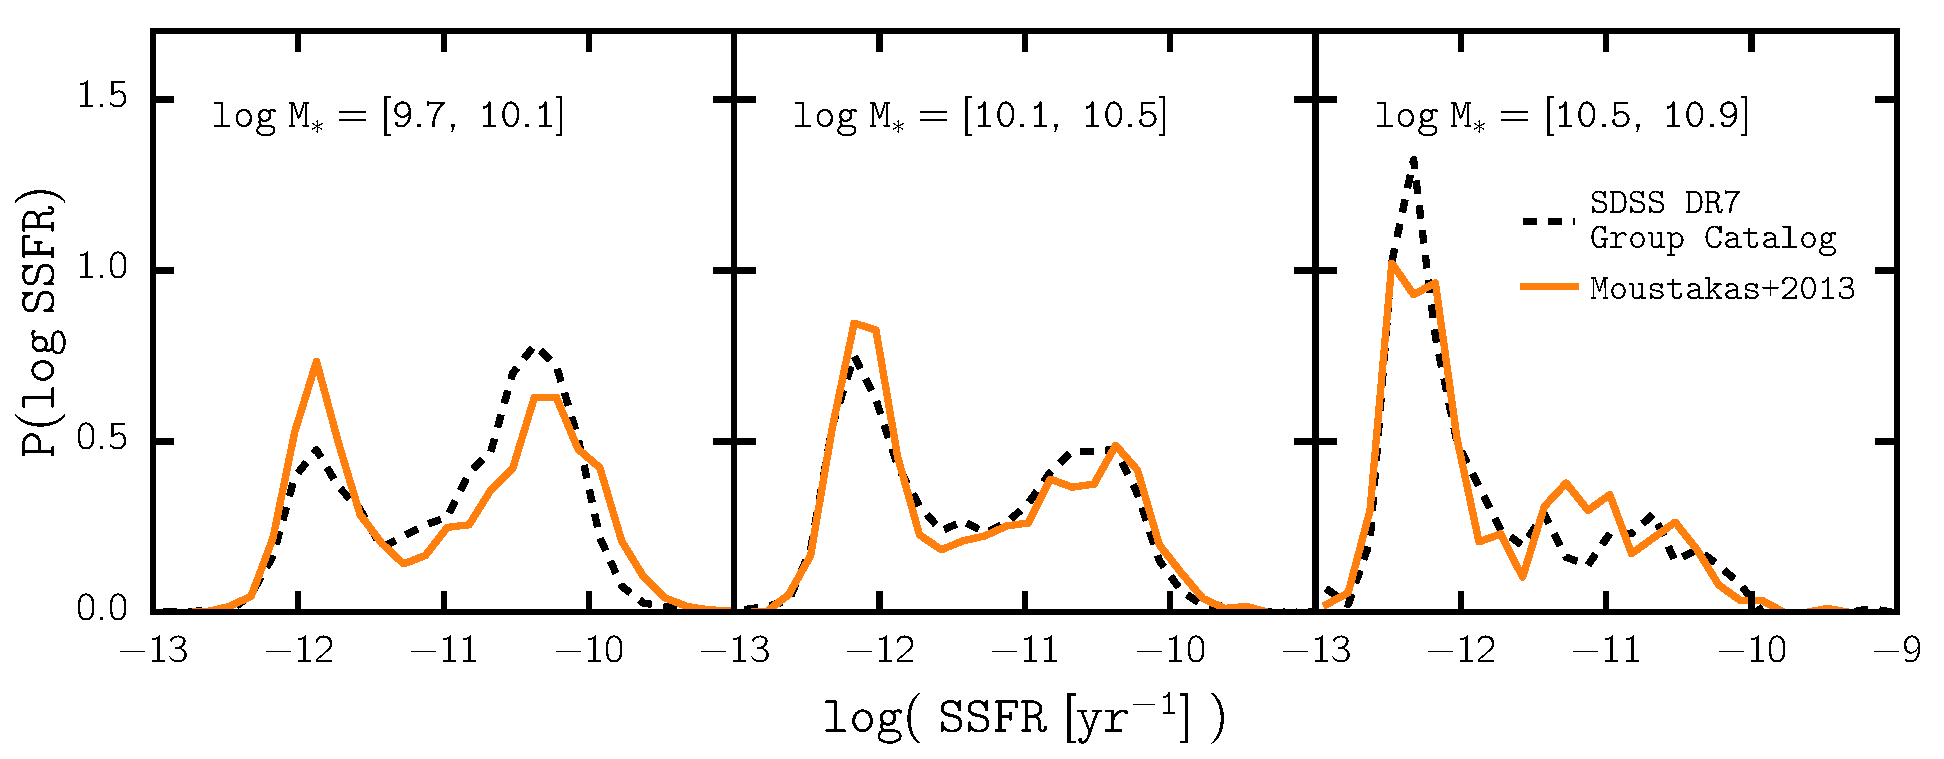
\includegraphics[width=\textwidth]{figs/cenq/Pssfr_comparison.pdf}
\caption{
Comparison of the SSFR distribution calculated using 
SSFRs from the SDSS DR7 group catalog (black dashed) versus
\cite{Moustakas:2013aa} (orange) for galaxies that are in 
both the SDSS DR7 group catalog and the \cite{Moustakas:2013aa} 
sample $z\sim0.1$ bin: $P(\mathrm{SSFR}^{\rm group})$ versus 
$P(\mathrm{SSFR}^{M2013})$. Galaxies are binned based on the
group catalog $\mathcal{M}_*$ for both distributions so that 
the same galaxies are examined in each bin. We impose SSFR 
bounds on $P(\mathrm{SSFR}^{M2013})$ for low SSFRs to reproduce 
the $P(\mathrm{SSFR}^{\rm group})$ quiescent peak (\S~\ref{sec:sdss}). 
We note that the M2013 sample does not contain a large number 
of galaxies within the group catalog's $z$ range at higher 
mass bins due its bright magnitude limit.
We find good overall agremeent between $P(\mathrm{SSFR}^{\rm group})$ 
and $P(\mathrm{SSFR}^{M2013})$. Furthermore, they have consistent 
green valley heights, which is the main feature of $P(SSFR)$ critical 
for constraining the central quenching timescale.
}
\label{fig:Pssfr_comp}
\end{center}
\end{figure*}



%%%% Bibliography %%%%%%%%%%%%%%%
\clearpage
\addcontentsline{toc}{chapter}{Bibliography}
\bibliography{thesis}


\end{document}
